\documentclass[]{article}
\usepackage[a4paper, margin=2cm]{geometry}
\usepackage{multicol}

\usepackage{cite}
\usepackage{hyperref}
\usepackage{caption}
\usepackage{graphicx}
\graphicspath{{./images/}}
\newenvironment{Figure}
{\par\medskip\noindent\minipage{\linewidth}}
{\endminipage\par\medskip}

\title{Deep Learning Fall 2019 Project Report\\\large{Large, Random Non-trainable Layers in Neural Networks with Memory Constraints}}
\author{Bram van den Heuvel \& Matej Sladek}

\pagestyle{empty}

\begin{document}

\maketitle

\begin{abstract}
	In this project we present approach to implement non-trainable layers in regards of memory usage and we evaluate effect on performance and training stability after adding random layers to different architectures. The performance was not improved after adding random layers and training stability was improved in one classification task.
\end{abstract}


\begin{multicols}{2}
	\section{Introduction}
	Classical statistics suggests there is a paradox going on in deep learning: the models have an enormous number of parameters, but they do not suffer from the downsides of that fact the same way that virtually all other model classes do.
	
	In the early 1990's, Schmidt et. al. \cite{Schmidt_Kraaijveld_Duin} attempted to explain this phenomena by showing that many of the parameters in a deep model are of less importance. They describe how the first layers of a neural net can be viewed as a collection of nonlinear features of the input data, with a simple linear regression attached to it in the final layer. The weights in the final layer are of higher importance. They demonstrate this by randomly initializing some of the hidden layers with random weights and keeping their values fixed throughout the training procedure. We call these layers \emph{random layers}. The training procedure still works surprisingly well.
	
	The value of depth and a large number of parameters is demonstrated by the models performing best in the ImageNet Large Scale Visual Recognition Challenge (INLSVRC) \cite{DBLP:journals/corr/CanzianiPC16}. In the last decade, the number of layers in the top-performing model has gone up to 152 with ResNet. Also the number parameters has grown; models often use tens of millions of parameters, VGG-19 as much as 155 million. This translates to a maximum memory usage during training of approximately 200 MB for most models, a little over 800 MB for VGG-19, when trained with a batch size of one. This then increases to above 1000 MB for several top-performing models once the batch is increased to 16, and increases approximately linearly with batch size beyond that. This means that with a batch size of 64, none of the top performing models can be trained on a mobile device or a consumer-grade GPU because of memory limitations.
	
	Our contribution is proposal for memory effective non-trainable random layers and performance and training stability evaluation of architectures with added random layers and comparison them with architectures without random layers.
	
	\section{Models and Methods}
	We study the effect of introducing new random layers, or replacing existing layers by random layers. We propose idea to store weights of random layer in memory effective way. We do not have the means to provide an implementation of our idea. We measure model performance exactly by simply storing the random layers completely.
	
	\subsection{Idea}
	Idea description
	
	
	\subsection{Performance}
	To measure the effect of random layers on performance we identified the following tasks:
	\begin{itemize}
		\itemsep0em
		\item Convolutional architecture to classify images from the MNIST fashion dataset
		\item Dense architecture to classify level of income on the census income dataset
		\item Dense architecture to do regression on the census income dataset
		\item Run bayesian optimization to identify best model architecture with possibility of random layers and cap on trainable parameters
	\end{itemize}
	For MNIST dataset we evaluate 3 dense architectures, 3 convolution architectures with one convolution, max pooling and varying number of dense layers, 3 convolution architectures with added varying number of random layers.

	For census income dataset we evaluate dense models without random layer, with 1 random layer and with 2 random layers. Every of this configuration we train with multiple sizes of layers before and after random layer. We also evaluate architecture with residual random layers where we can train one scalar for random layer or one scalar for every node of random layer.
	
	In optimization, domain of search is size of random layer, number of random layers, size of end layer, activation function of random layer, activation of last layer and whether use batch norm.	
	
	For the training we use Adam optimizer and early stopping callback to stop learning after evaluation loss does not change much.
	
	\section{Results}
	On MNIST dataset we data to training and test data set in ratio 8:1. We train every architecture one time. The loss function is sparse categorical crossentropy (higher is better). Best dense configuration had performance 0.89\%, best convolution configuration had 0.91\% and with added random layers best performance was 89\%. In (Fig 1) can be seen plot with data point for every configuration. On plot we see means of every type of architecture. After adding random layers the performance dropped.
	
	On Census income we use K-fold evaluation and we split data to 10 parts and every architecture configuration train for 10 times. In regression task loss is mean squared error(lower is better). In (Fig 2) we can see that mean of results is similar even if we add 1 or 2 random layer. We also go deeper with random layers with using residual random layers. We evaluate architectures with 10, 20, 30 and 40 residual random layers. Results are in (Fig 3) and there are not much difference when we add more random layers.
	
	On Census income on classification task we take same models as in regression. We use sparse categorical crossentropy loss. Results are in (Fig 4). Best models have similar results even after adding random layer, but we can see mean is smaller for architectures without random layer and that is because few models has low performance, so we can see that stability of training went up after adding random layer.	
	
	\section{Discussion}
	From results we can say that adding few random layers does not improve performance. Mean performance of models went a little bit down after adding these layers. Same happen when we add lots of residual random layer. In classification task of census income models without any random layer happened have lower performance in some cases, but after adding random layer we have not see it. From that we conclude that in some cases random layers can improve stability of training.
	
	\begin{Figure}
		\centering
		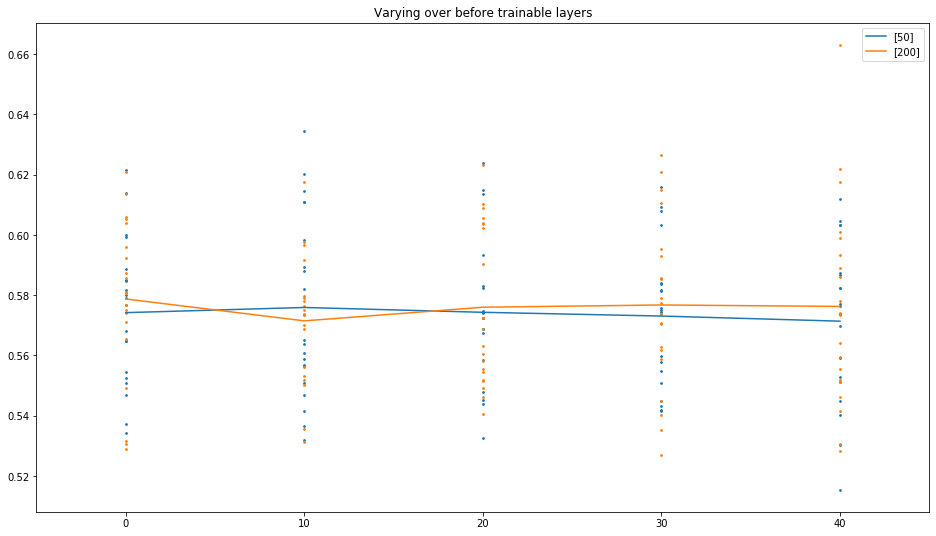
\includegraphics[width=\linewidth]{index.png}
		\captionof{figure}{Abc}
		\label{fig:result}
	\end{Figure}
	
	\section{Summary}
	In conclusion we proposed idea to memory limited implementation of random layers. We evaluated models with or without random layers on regression and classification tasks. We conclude that adding random layers does not change performance a much. In evaluation of classification task of census income dataset, we have seen that training stability was improved.
	
	\bibliography{../bibliography}
	\bibliographystyle{plain}
\end{multicols}

I refer to the image \ref{fig:result}.

\end{document}
